% @author Arian Helberg

\chapter{Evaluierung}
\label{eval}
Die Synthese von Verzweigungstrukturen wird in den vorangegangenen Kapiteln konzeptionell betrachtet
und in einem Softwareprojekt umgesetzt.
Im Folgendem werden Teilaspekte an einem fortlaufenden Beispiel evaluiert und bewertet.
Diese Aspekte umfassen:
\begin{itemize}
    \item das Nutzen von Templates
    \item die Erstellung und Visualisierung von Verzweigungsstrukturen
    \item Aufbau einer Baumstruktur
    \item Extrahierung von Regeln und Mustern
    \item Komprimierung von L-Systemen
    \item Erweiterung von L-Systemen
    \item Synthese von Ähnlichkeitsstrukturen
    \item Auswirkung der Gewichtungsparameter
\end{itemize}

\subsection*{Templates}
Die Nutzung von Templates als Terminale einer Grammatik findet Anwendung in vielen wissenschaftlichen Arbeiten.
\citeauthor{aliaga_2016} liefert hierzu eine umfassende Übersicht~\cite{aliaga_2016}.
Mit der Verwendung einer allgemeinen Repräsentation mithilfe von \textit{turtle}-Befehlen, wird eine
Wiederverwendbarkeit der genutzten Templates sichergestellt.
Die in dieser Arbeit erstellte Software nutzt ein minimalistisches System zum Einlesen der Templates aus
einer textbasierten Datei.
Die Forschung zur inversen prozeduralen Modellierung zeigt wiederum den Einsatz von
neuronalen Netzen als vielversprechende Methode Strukturen zu erkennen und Regeln abzuleiten.\\
Während neuronale Netze eine Eingabestruktur analysieren und in einer baumähnlichen Struktur organisieren,
knüpft diese Arbeit hier an und nutzt aus Praktikabilitätsgründen stattdessen eine benutzergeführte Anordnung
von Templates zu einer Verzweigungsstruktur.\\~\\
\underline{Beispiel}: Die Template-Zeichenketten haben folgende Form:
\begin{figure}[H]
    \centering
    \begin{csource}
    FX
    F-FX
    F+FX
    F[-FX]+FY
    F[-FX]FY
    F[FX]+FY
    F[-FX][FY]+FZ
    F[+FX]F[-FY]FZ
    \end{csource}
    \caption{templates.txt}
\end{figure}
\textit{F}, \textit{-}, \textit{+}, \textit{[} und \textit{]} sind aus dem Turtle-Algorithmus bekannte
Befehlssymbole.
Alle anderen Symbole (z.B. \textit{X, Y, Z}) stellen Verzweigungsvariablen dar, um anzuzeigen, an welcher Stelle
der Templatestruktur eine neue Verzweigung abgehen kann.

\subsection*{Erstellung und Visualisierung}
Durch die Ausführung bestimmter \textit{turtle}-Befehle der template-basierten Struktur, wird diese visualisiert.
Deshalb bietet es sich an, einfache grafische Elemente zu nutzen, um Verzweigungsstrukturen sichtbar zu machen
(z.B. Canvas).
Das Programm nutzt stattdessen interaktive Elemente innerhalb eines JavaFX Pane gegenüber statischen Elementen, um
die Strukturen zu zeichnen.
Der Prozess der Erstellung ist benutzergeführt und muss somit interagierbar sein.
So können Elemente genutzt werden, mit denen der Benutzer kommunizieren kann (z.B. klickbare Kreise).
Es ist nun möglich Verzweigungsstrukturen in einem simplen Arbeitsablauf zu erstellen.

\newpage

\underline{Beispiel}: Aus der Erstellung der Verzweigungsstruktur ergibt sich folgende Abbildung:
\begin{figure}[H]
    \centering
    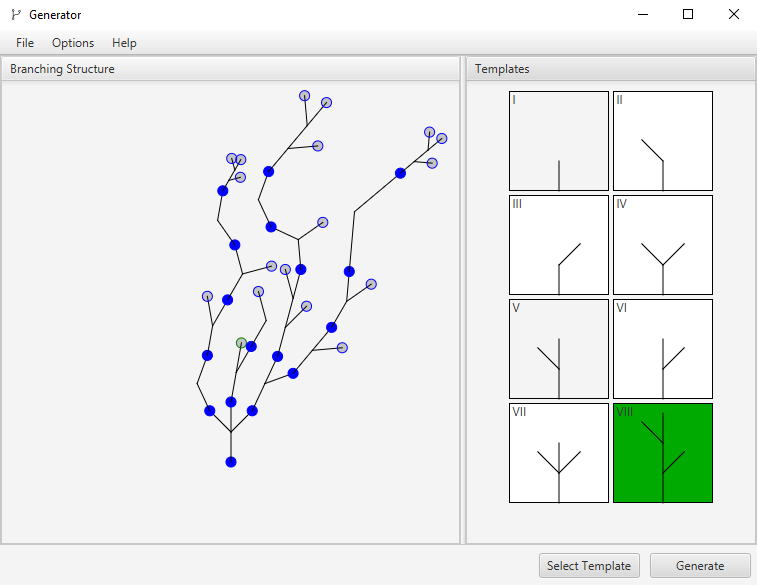
\includegraphics[width=12cm]{../images/evaluierung_inferrieren.png}
    \caption{Grafische Benutzeroberfläche nach der Erstellung einer Basisstruktur}
\end{figure}

\subsection*{Aufbau einer Baumstruktur}
Baumähnliche Strukturen eignen sich gut, um Tansformationsparameter und topolo-gische Anordnung von Templates
datenstrukturell zu trennen.\\
Ein ganzheitlicher Ansatz zur Analyse von Verzweigungsstrukturen ist die Kombina-tion aus Strukturtopologie und
räumlichen Transformationen.
Ein weiterer Ansatz ist die separate Betrachtung von Topologie und Transformation.
Beide Ansätze sind derzeit Gegenstand der Forschung.\\
Das von \citeauthor{benes_2011} vorgestellte System nutzt beispielsweise einen ganzheitlichen Ansatz, um sog.
\textit{Guides} zu erstellen, welche Teilsysteme der Eingabestruktur beschreiben.
Hier unterscheiden sich Strukturen, die zwar identische Verzweigungen aufweisen, jedoch deren
Transformationsparameter (z.B. der Winkel von Verzweigungen) voneinander abweichen.
Auch in der Arbeit von \citeauthor{stava_2010} zeigt sich eine Organisation von
"`Clustern"' mit Transformationen, die in eine Signifikanzbewertung einfließen~\cite{stava_2010}.

\newpage

Bei einer separaten Betrachtung von Topologie und Transformation zeigen \citeauthor{nishida_2016} und \citeauthor{guo_2020},
dass es sinnvoll ist zwei spezialisierte, neuronale Netze zu verwenden, da die räumlichen Transformationen das Erkennen
der Topologie nicht signifikant beeinflussen~\cite{nishida_2016, guo_2020}.\\
Diese Arbeit legt den Fokus auf die datenstrukturelle Trennung von \mbox{Transformationen} und topologischer
Anordnung und erstellt somit eine Baumstruktur, die Template-Instanzen als Knoten und
räumliche Transformationen als eingehende Kanten darstellt.\\~\\
\underline{Beispiel}: Aus der Eingabestruktur ergibt sich folgender Baum (die räumlichen Transformationen sind hier nicht visualisiert):
\begin{figure}[H]
    \centering
    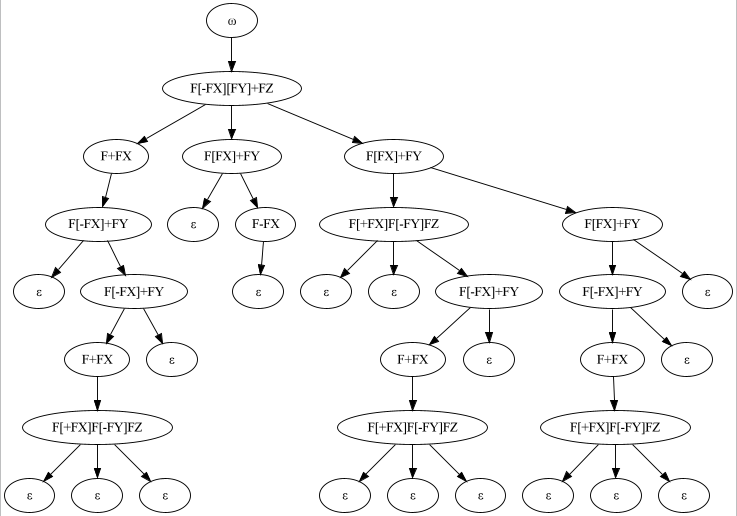
\includegraphics[width=12cm]{../images/evaluierung_inferrieren_baum.png}
    \caption{Baumstruktur der erstellten Verzweigungsstruktur}
\end{figure}

\subsection*{Extrahieren von Regeln und Mustern}
Die in~\ref{alg2} vorgestellte Methodik zum Inferieren eines L-Systems aus einer Baumstruktur
stellt einen Algorithmus vor, der auf die spezielle Baumstruktur zugeschnitten ist.
Die L-Systeme entsprechen lediglich der Eingabestruktur und beinhalten keine Transformationen.\\~\\
\underline{Beispiel}: Ausgeführte Ersetzungssysteme werden über einen JavaFX Dialog visualisiert:
\begin{figure}[H]
    \centering
    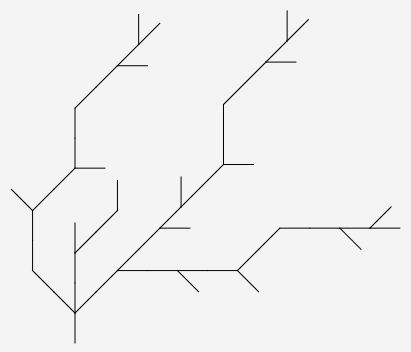
\includegraphics[width=8cm]{../images/evaluierung_inferrieren_lsystem.png}
    \caption{Inferiertes L-System}
\end{figure}
Die Zeichenkettenrepräsentation des L-Systems ($\mathcal{L}=\{M,\omega,R\}$) lautet:
\begin{csource}
LSystem{
    [F, S, A, B, C, D, E, G, H, I, J, K, L, M, N, O, P, Q, R, T, U, V, W, X, Y, Z, a, b, c, d, e, f, g, h, i, j, k],
    S,
    [S -> A, A -> F[-FB][FC]+FD, B -> F+FE, C -> F[FG]+FH, D -> F[FI]+FJ, E -> F[-FK]+FL, G -> _, H -> F-FM, I -> F[+FN]F[-FO]FP, J -> F[FQ]+FR, K -> _, L -> F[-FT]+FU, M -> _, N -> _, O -> _, P -> F[-FV]+FW, Q -> F[-FX]+FY, R -> _, T -> F+FZ, U -> _, V -> F+Fa, W -> _, X -> F+Fb, Y -> _, Z -> F[+Fc]F[-Fd]Fe, a -> F[+Ff]F[-Fg]Fh, b -> F[+Fi]F[-Fj]Fk, c -> _, d -> _, e -> _, f -> _, g -> _, h -> _, i -> _, j -> _, k -> _]
}
\end{csource}

Das inferierte L-System zeigt, dass die Eingabestruktur richtig in eine Grammatik überführt wurde.
Dabei steht der Unterstrich (\_) für das leere Wort $\varepsilon$ und damit für die leeren Knoten
der aufgebauten Baumstruktur.

\subsection*{Komprimieren des L-Systems}
Die Zeichenkettenrepräsentation des inferierten L-Systems zeigt einige Redundanzen auf.
Zum Beispiel bilden
\begin{csource}
    P -> F[-FF+FF[+F]F[-F]F]+F
\end{csource}
und
\begin{csource}
    Q -> F[-FF+FF[+F]F[-F]F]+F
\end{csource}
das gleiche Muster.
Um solche Redundanzen zu entfernen, wird das L-System in der vorgestellten Komprimierungs-Pipe reduziert.
Hierbei werden identische, maximale\\Unterbäume und deren leere Kindknoten zusammengefasst.
Der Gewichtungsparameter für das Beispiel wird auf 0.5 gesetzt.
Es ergibt sich folgender Baum:
\begin{figure}[H]
    \centering
    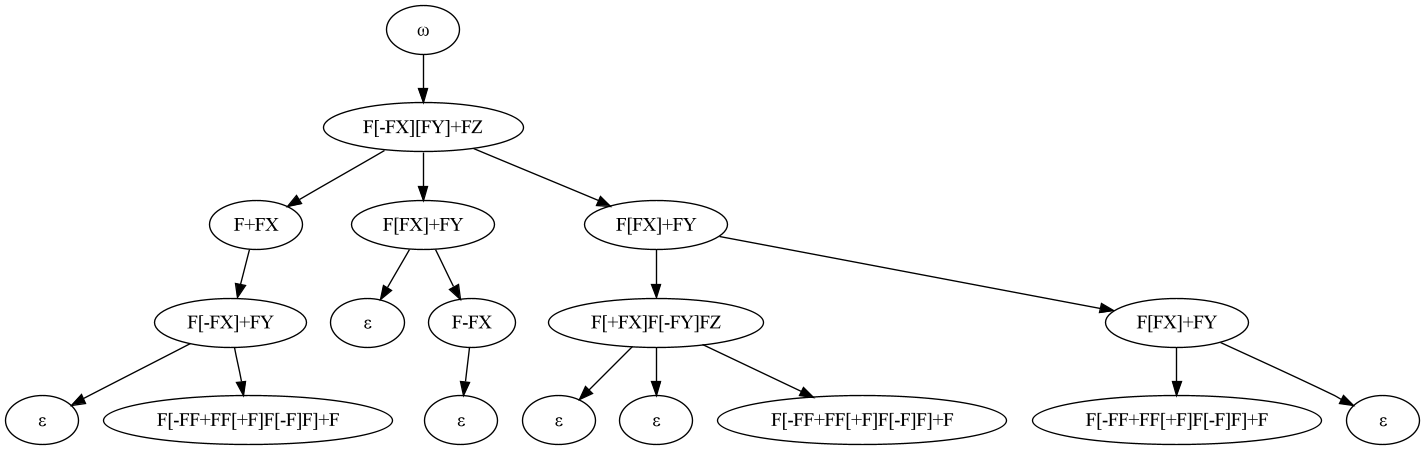
\includegraphics[width=14cm]{../images/compressed_tree.png}
    \caption{Komprimierter Baum}
\end{figure}

Die Baumstruktur zeigt, dass der Komprimierungsalgorithmus die maximalen Subbäume erfolgreich reduziert.
Das komprimierte L-System setzt sich wie folgt zusammen:
\begin{csource}
LSystem{
    [F, S, A, B, C, D, E, G, H, I, J, K, L, M, N, O, P],
    S,
    [S -> A, A -> F[-FB][FC]+FD, B -> F+FE, C -> F[FG]+FH, D -> F[FI]+FJ, E -> F[-FK]+FL, G -> _, H -> F-FM, I -> F[+FN]F[-FO]FP, J -> F[FL]+FG, K -> _, L -> F[-FF+FF[+F]F[-F]F]+F, M -> _, N -> _, O -> _, P -> F[-FF+FF[+F]F[-F]F]+F]
}
\end{csource}

\subsection*{Generalisieren des L-Systems}
Der vorgestellte Generalisierungsalgorithmus verändert das L-System der Eingabestruktur, indem
Produktionsregeln miteinander verbunden und mit einer Wahrscheinlichkeit versehen werden.
Der Gewichtungsparameter wird für das Beispiel auf 0.5 gesetzt.
Es ergibt sich das finale L-System:
\begin{csource}
LSystem{
    [F, S, E, G, K, M, N, A],
    S,
    [S -> A, E -> F[-FK]+FA, G -> _, K -> _, M -> _, N -> _, A -> F-FM, A -> F[-FA][FA]+FA, A -> F[FG]+FA, A -> F[FA]+FG, A -> F+FE, A -> F[+FN]F[-FA]FA, A -> F[-FF+FF[+F]F[-F]F]+F, A -> F[FA]+FA, A -> _]
}
\end{csource}

Die Produktionsregelmenge zeigt einige Regeln auf, die dasselbe Ziel haben.
Sie werden bei ihrer Anwendung zufällig ausgewählt.


\subsection*{Synthese}
Führt man das generalisierte L-System aus, ergeben sich die Ähnlichkeitsstrukturen.
Eine Evaluierung wird stichprobenartig durchgeführt, erweist sich jedoch als schwierig, da
es bei der Erstellung der Ausgabestrukturen um Wahrscheinlichkeiten beim Auftreten gewisser
Muster handelt.
Da die Algorithmen eine akzeptable Lösung eines schwierigen Problems liefern sollen,
ist die Bewertung der Ergebnisse subjektiv.
\begin{figure}[H]
    \centering
    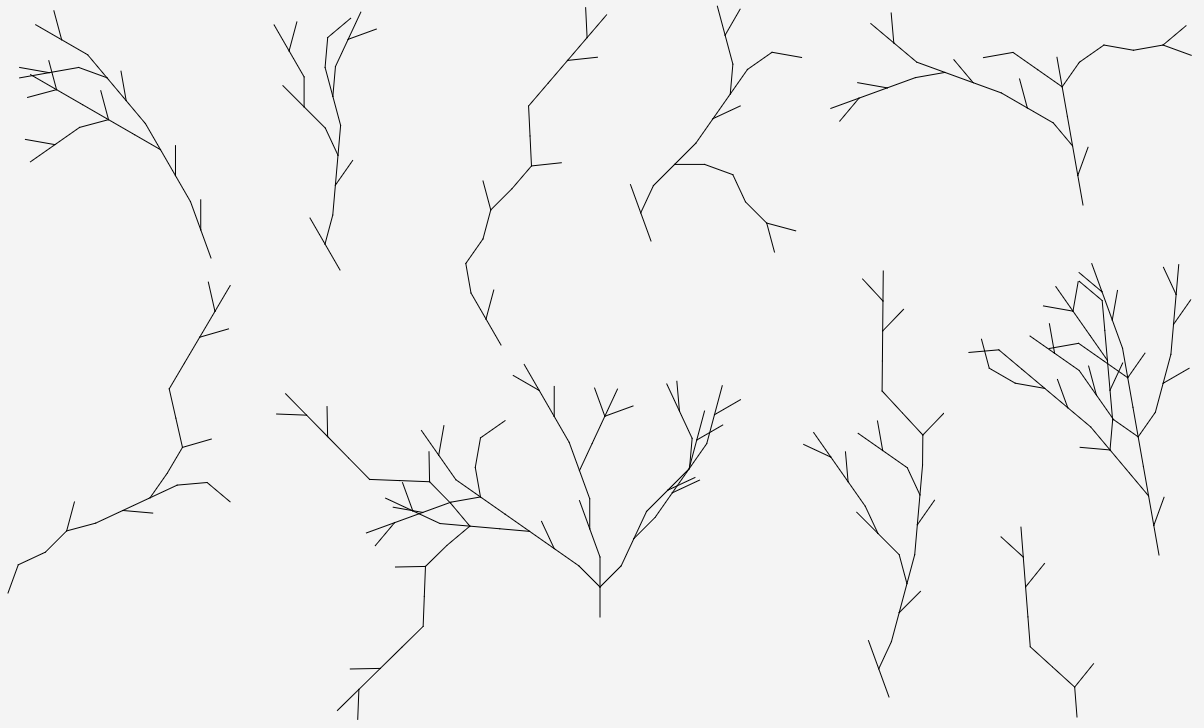
\includegraphics[width=14.5cm]{../images/synthesis.png}
    \caption{Synthetisierte Verzweigungsstrukturen}
\end{figure}

Vergleicht man die Eingabestruktur mit den synthetisierten Strukturen, weisen diese
gewisse Eigenschaften auf (siehe folgende Abbildung):
\begin{itemize}
    \item Wiederholtes Auftreten einer Struktur, die beim Synthetisieren als maximaler\\Unterbaum
    erkannt wurde (rot)
    \item Anwendung von benutzerdefinierten Transformationsparametern (blau)
    \item Ähnliche Häufigkeiten (grün)
    \item Isoliertes Auftreten von Templates des maximalen Subbaums, die über den Unterbaum
    hinaus einzeln vorkommen (gelb)
\end{itemize}

\begin{figure}[H]
    \centering
    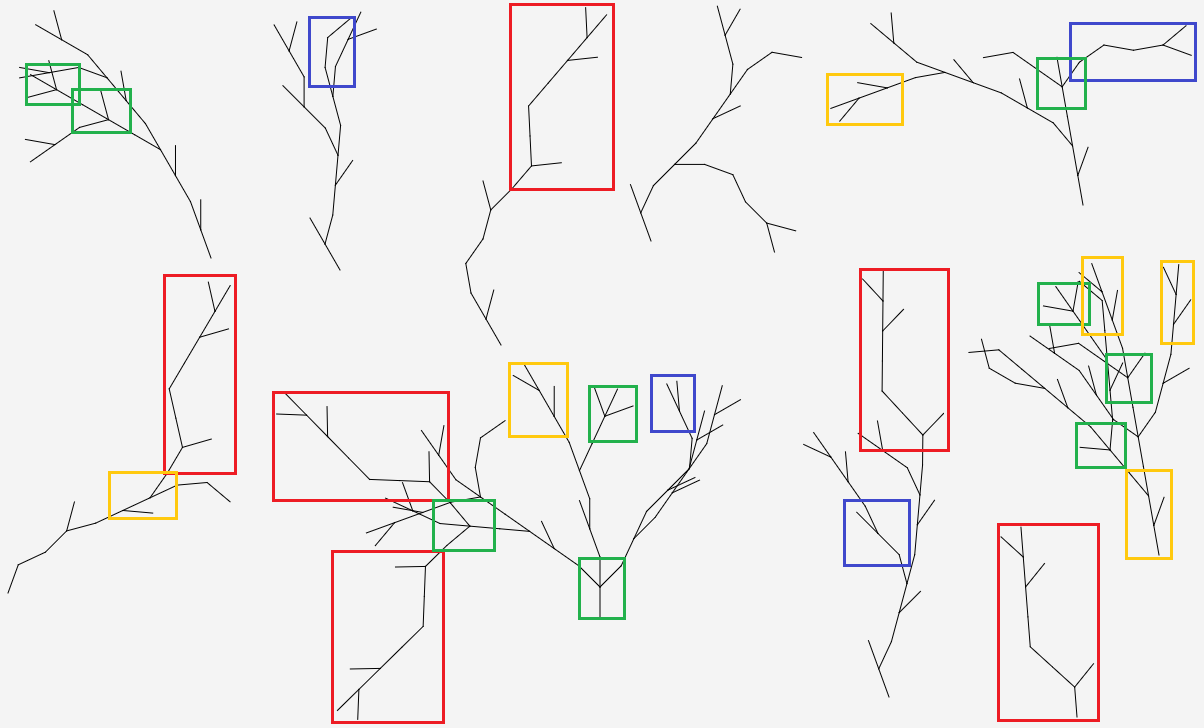
\includegraphics[width=14.5cm]{../images/synthesis_marks.png}
    \caption{Untersuchung der synthetisierten Verzweigungsstrukturen}
\end{figure}

\subsection*{Auswirkung der Gewichtungsparameter}
Der Parameter $w_l$ des vorgestellten Komprimierungsalgorithmus gewichtet eine Funktion,
welche die Kosten eines L-Systems ermittelt, sodass der Algorithmus L-Systeme mit unterschiedlich
großer Produktionsregelmenge anders behandelt.
Hierbei bewertet ein Wert von $0.0$ eine große Produktionsregelmenge höher.
Entspricht $w_l$ einem Wert von $1.0$, wird eine kleinere Produktionsregelmenge überbewertet.
Der Durchschnittswert $0.5$, der im Beispiel verwendet wird, sorgt für eine moderate Menge an
Produktionsregeln bei moderater Länge der einzelnen Regel.
Der im Generalisierungsalgorithmus vorgestellte Gewichtungsparameter $w_0$ legt fest, inwiefern
die Länge oder \textit{String Edit Distance} zweier Grammatiken von Bedeutung sind.
Bei einem Wert von $0.0$ überbewertet der Algorithmus die Metrik zur Berechnung der Anzahl Operationen,
um eine Grammatik in eine zweite zu überführen.
Der Wert $1.0$ entspricht einer Überbewertung der Längenmetrik.
Im Beispiel wird der Durchschnittswert $0.5$ verwendet.

$w_l$ und $w_0$ sind im Programm als \textit{Rula application ratio} und \textit{Merge application ratio}
bezeichnet und können vom Benutzer vor der Generierung festgelegt werden.